\section{Lösung}
\textbf{zu Aufgabe \ref{AufgVor7}}

Es sollen Abstände auf einem Werkstück mit Hilfe eines induktiven Wegaufnehmers gemessen werden.
Das Messprinzip eines induktiven Wegaufnehmers beruht darauf, dass
eine Wechselspannung ein Spulensystem im Sensor anregt.
Ein bewegliches ferro-magnetisches Teil am Sensor
beeinflusst die Induktivität in den Spulen.
Diese - in den Spulenteilen unterschiedliche - Induktivitätsveränderung wird vom
Messverstärker ausgewertet und in ein positions-proportionales Gleichspannungssignal
umgewandelt.

Um die Abstände in der physikalischen Einheit Mikrometer zu erhalten, muss mit Hilfe
eines Bezugsnormals aus dem Spannungssignal ein Weg mit der Dimension einer Länge
berechnet werden.
Es ist bekannt, dass in dem für die Messung relevanten Messbereich (Hub des Sensors)
die Abhängigkeit zwischen Spannungssignal und Auslenkung des ferro-magnetischen Kerns
linear ist.
Das Bezugsnormal ist eine Stufenhöhe.

Zu dem Bezugsnormal gibt es einen Kalibrierschein, der folgenden Höhenwert für das
Normal angibt:
\begin{equation}
d \; = \; (4.997 \pm 0.011) \; \mathrm{\mu m} \qquad \mathrm{mit} \qquad k = 2.1, \nu_d = 26
\label{eq:kalBezug}
\end{equation}

Mit dem induktiven Wegaufnehmer wurden auf dem Bezugsnormal folgende Stufenhöhen in
der Dimension der elektrischen Spannung mit der Einheit Millivolt gemessen

% muB = 200; sigB = 8;
% JB = 11; xB = muB+sigB*randn(1,JB);
% printf("& %4.1f ", xB);
% xB = [201.3  187.3  196.5  200.4  193.6  174.2  197.2  185.4  194.4  202.5  205.2];
Tabelle A5.1:\\
\begin{tabular}{c||c|c|c|c|c|c|c|c|c|c|c}
\hline
$U_\mathrm{B} / \mathrm{mV}$ & 201.3 & 187.3 & 196.5 & 200.4 & 193.6 & 174.2 & 197.2 & 185.4 & 194.4 & 202.5 & 205.2\\
\hline
\end{tabular}

%Für den Abstand auf dem Werkstück wurden folgende Spannungen gemessen
%>> muW = 180; sigW = 11;
%>> JW = 7; xW = muW+sigW*randn(JW,1);
%>> printf(" %4.1f ", xW);
% 176.5  184.1  180.5  193.6  176.0  194.5  160.9 >>
%>> printf("& %4.1f ", xW);
Tabelle A5.2:\\
\begin{tabular}{c||c|c|c|c|c|c|c}
\hline
$U_\mathrm{W} / \mathrm{mV}$ & 176.5 & 184.1 & 180.5 & 193.6 & 176.0 & 194.5 & 160.9 \\
\hline
\end{tabular}

Der Zusammenhang zwischen dem Abstand auf dem Werkstück in Mikrometern $d_\mathrm{W}$,
der Stufenhöhe des Bezugsnormals gemäß Kalibrierschein $d$, dem gemessenen Spannungssignal
an der Stufenhöhe $U_\mathrm{B}$ und dem gemessenen Spannungssignal $U_\mathrm{W}$ am Werkstück
ist folgender
\begin{equation}
d_\mathrm{W} \; = \; \frac{d}{U_\mathrm{B}} \, U_\mathrm{W}
\end{equation}

Die Änderungen aufgrund der statistischen Streuung der Spannungswerte $U_\mathrm{B}$ sind
so klein, dass für die Sensitivität $c_\mathrm{B}$ von $d_\mathrm{W}$
bezüglich Änderungen von $U_\mathrm{B}$
mit dem hyperbolischen Zusammenhang $d_\mathrm{W} \sim \frac{1}{U_\mathrm{B}}$
die Steigung der Tangenten an die Hyperbel verwendet wird. Es wird die
Tangente verwendet, die an dem Punkt, der sich aus den Mittelwerten
ergibt, anliegt.
\begin{equation}
c_\mathrm{B} \; = \; \left. \frac{\partial}{\partial U_\mathrm{B}}
 d_\mathrm{W} \right|_{\bar U_\mathrm{B}, \bar d, \bar U_\mathrm{W}}
\end{equation}
Die Sensitivitäten $c_\mathrm{d}$ und $c_\mathrm{W}$ von $d_\mathrm{W}$
bezüglich Änderungen von $d$ und $U_\mathrm{W}$ sind aufgrund des
linearen Zusammenhangs genau
\begin{equation}
c_\mathrm{d} \; = \; \left. \frac{U_\mathrm{W}}{U_\mathrm{B}} \right|_{\bar U_\mathrm{B}, \bar U_\mathrm{W}} \qquad
c_\mathrm{W} \; = \; \left. \frac{d}{U_\mathrm{B}} \right|_{\bar U_\mathrm{B}, \bar d}
\label{AufgPartiellLinear}
\end{equation}
definiert.
Die kombinierte Varianz unter der Voraussetzung, dass die gemessenen Größen und
die Angabe aus dem Kalbrierschein unkorreliert sind, ist
\begin{equation}
s_\mathrm{dW}^2 \; = \; (c_\mathrm{d} \, s_\mathrm{d})^2 \; + \;
(c_\mathrm{B} \, s_\mathrm{B})^2 \; + \; (c_\mathrm{W} \, s_\mathrm{W})^2
\end{equation}
mit $s_\mathrm{B}$ für die Standardabweichung der in Tabelle A5.1 aufgelisteten Werte,
$s_\mathrm{W}$ für die Standardabweichung der in Tabelle A5.2 aufgelisteten Werte und
$s_\mathrm{d}$ für die Standardabweichung der Angabe aus dem Kalibrierschein.

\begin{itemize}
\item[a)] Ermitteln Sie aus den Angaben des Kalibrierscheins (hier Gl.~(\ref{kalBezug}))
die Standardabweichung $s_\mathrm{d}$, indem Sie den dort genannten Erweiterungsfaktor verwenden.
%>> d = 4.997 d =  4.9970

Die im Kalibrierschein angegebene erweiterte Messunsicherheit $U(d)\, = \, k s_\mathrm{d}$
beträgt $0.011 \, \mathrm{mu m}$. Um an die Standardabweichung $s_\mathrm{d}$ zu kommen,
die in die Unsicherheitsfortpflanzungsformel einzusetzen ist,
muss durch den Erweiterungsfaktor $k = 2.1$ geteilt werden:
%>> sd = 0.011/2.1 sd =  0.0052381
$$
s_\mathrm{d} = \frac{0.011 \, \mathrm{\mu m}}{2.1} = 0.00524 \; \mathrm{\mu m}
$$
\item[b)] Ermitteln Sie die beiden Mittelwerte $\bar U_\mathrm{B}$ und $\bar U_\mathrm{W}$,
sowie die beiden empirischen Standardabweichungen $s_\mathrm{B}$ und $s_\mathrm{W}$
aus den beiden Tabellen A5.1 und A5.2.
%>> xBbar = mean(xB) xBbar =  194.36
%>> xWbar = mean(xW) xWbar =  180.85
%>> sW = std(xW) sW =  11.561
%>> sW2 = var(xW) sW2 =  133.65
%>> sB = std(xB) sB =  9.0410
%>> sB2 = var(xB) sB2 =  81.739
$$
\bar U_\mathrm{B} \, = \, \frac{1}{J_\mathrm{B}}\sum\limits_{j=1}^{J_\mathrm{B}}  U_{\mathrm{B},j}
\, = \, 194.364 \; \mathrm{mV},
\quad
 s_\mathrm{B}  = \sqrt{\frac{1}{J_\mathrm{B}-1}\sum\limits_{j=1}^{J_\mathrm{B}}} \, = \,
 9.045 \; \mathrm{mV}
$$
mit $J_\mathrm{B} = 11$ und
$$
\bar U_\mathrm{W} \, =  \, \frac{1}{J_\mathrm{W}}\sum\limits_{j=1}^{J_\mathrm{W}}  U_{\mathrm{W},j}
\, = \, 180.871 \; \mathrm{mV}, \quad s_\mathrm{W}  =  11.547 \; \mathrm{mV}
$$
mit $J_\mathrm{B} = 7$.

\item[c)] Bestimmen Sie die Sensitivitäten $c_\mathrm{d}$, $c_\mathrm{W}$, $c_\mathrm{B}$ durch Ausführen der
partiellen Ableitung.
%(%i4) dW(UB) := UW*d/UB;
%                                          UW d
%(%o4)                           dW(UB) := ----
%                                           UB
%(%i5) diff(dW(UB),UB);
%                                      d UW
%(%o5)                               - ----
%                                        2
%                                      UB
Mit 
\begin{equation*}
c_\mathrm{d} \; = \; \left. \frac{U_\mathrm{W}}{U_\mathrm{B}} \right|_{\bar U_\mathrm{B}, \bar U_\mathrm{W}} \qquad
c_\mathrm{W} \; = \; \left. \frac{d}{U_\mathrm{B}} \right|_{\bar U_\mathrm{B}, \bar d}
\end{equation*}
gilt
$$
c_\mathrm{d} \; = \; \frac{\partial d_\mathrm{W}}{\partial d}
\; = \; \frac{\partial}{\partial d} \frac{d}{U_\mathrm{B}} \, U_\mathrm{W}
\; = \; \frac{U_\mathrm{W}}{U_\mathrm{B}} \; =  \; 0.9306
$$
weil $\frac{U_\mathrm{W}}{U_\mathrm{B}}$ bezüglich der Ableitung nach $d$ Konstanten sind und die Ableitung von $d$
nach $d$ Eins ist. Entsprechend ist der Faktor $\frac{d}{U_\mathrm{B}}$ bzgl der Ableitung nach $U_\mathrm{W}$ eine
Konstante und $U_\mathrm{W}$ nach $U_\mathrm{W}$ abgeleitet gleich Eins.
$$
c_\mathrm{W} \; = \; \frac{\partial d_\mathrm{W}}{\partial U_\mathrm{W}} \; = \; \frac{d}{U_\mathrm{B}} \; = \;  0.0257 \; \frac{\mathrm{\mu m}}{\mathrm{mV}}
$$
$$
c_\mathrm{B} \; = \; \frac{\partial d_\mathrm{W}}{\partial U_\mathrm{B}}
\; = \; \frac{\partial}{\partial U_\mathrm{B}} \frac{d}{U_\mathrm{B}} \, U_\mathrm{W}
\; = \; d \, U_\mathrm{W} \, \frac{\partial}{\partial U_\mathrm{B}} \frac{1}{U_\mathrm{B}}
\; = \; -\frac{d U_\mathrm{W}}{U_\mathrm{B}^2} \; = \;  -0.0239 \; \mathrm{\mu m}
$$
weil $d \, U_\mathrm{W}$ bzgl der Ableitung nach $U_\mathrm{B}$ eine Konstante und
$$
 \frac{\partial}{\partial U_\mathrm{B}} U_\mathrm{B}^{-1} = -U_\mathrm{B}^{-2}
$$
\item[d)] Berechnen Sie die kombinierte empirische Standardabweichung $s_{d,\mathrm{W}}$.
%>> cd = xWbar/xBbar cd =  0.93048
%>> cW = d/xBbar cW =  0.025710
%>> cB = -d*xWbar/(xBbar^2) cB = -0.023922
%s2 = (sd*cd)^2 + sW2*cW^2 + sB2*cB^2 s2 =  0.13514
%s = sqrt((sd*cd)^2 + sW2*cW^2 + sB2*cB^2) s =  0.36762
$$
s_{\mathrm{d},\mathrm{W}} \; = \; \sqrt{(c_\mathrm{d} \, s_\mathrm{d})^2 \; + \; (c_\mathrm{W} \, s_\mathrm{W})^2 \; + \; (c_\mathrm{B} \, s_\mathrm{B})^2} =    0.3674 \; \mathrm{\mu m}
$$
\item[e)] Berechnen Sie die effektive Anzahl der Freiheitsgrade.
%nueff = s2^2 / ((sd*cd)^4/26 + (sW2*cW^2)^2/(JW-1) + (sB2*cB^2)^2/(JB-1)) nueff =  12.019
$$
\nu_\mathrm{eff} \; = \; \frac{s_{\mathrm{d},\mathrm{W}}^4}{(c_\mathrm{d} \, s_\mathrm{d})^4/\nu_\mathrm{d} \, + \, (c_\mathrm{W} \, s_\mathrm{W})^4/(J_\mathrm{W}-1) \, + \, (c_\mathrm{B} \, s_\mathrm{B})^4/(J_\mathrm{B}-1)} \; = \; 12.04
$$
\item[f)] Berechnen Sie den Erweiterungsfaktor $k$, der
 hier das t-Quantil für ein zweiseitiges Vertrauensniveau
 von $1-\alpha = 0.95\%$ ist.

Berechnet mit Gnu-Octave:
\begin{verbatim}
 k=tinv(0.975,nueff) k =  2.1784
\end{verbatim}
$$
k = t_{0.975,12.04} = 2.178
$$
Für Ablesen aus der Quantilatabelle wird die effektive Anzahl der Freiheitsgrade abgerundet auf $\nu_\mathrm{eff} \, = \, 12$
und aus der Tabelle abgelesen:

\begin{center}
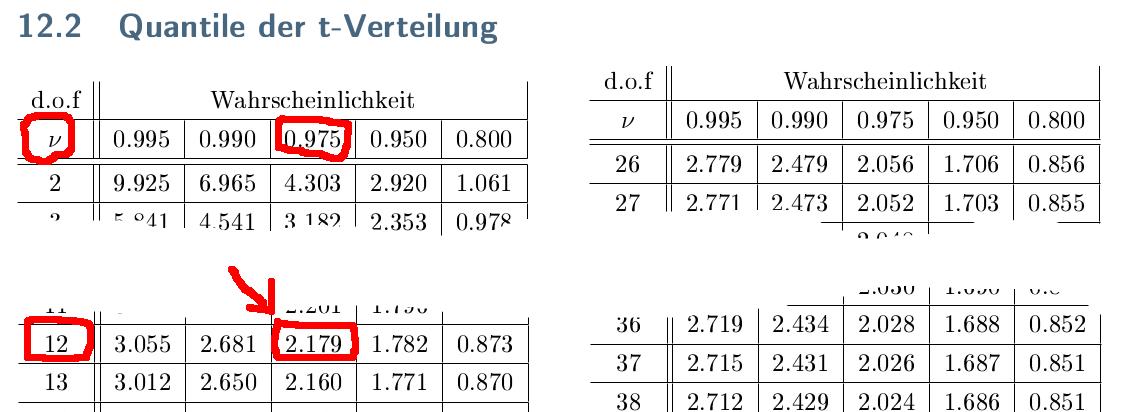
\includegraphics[width=95mm]{09_vorlesung/media/aufg_quantilaustabelle.png}
\end{center}

so dass dann folgender Wert verwendet wird
$$
k = t_{0.975,12.04} = 2.179
$$

\item[g)] Bestimmen Sie das vollständige Messergebnis.
% dW = d*xWbar/xBbar  dW =  4.6496
% k*s =  0.80083
% d_W = 4.6496 \pm 0.80083
$$
d_\mathrm{W} \; = \; \frac{d \, \bar U_\mathrm{B}}{\bar U_\mathrm{W}} \;  \pm \; k \, s_{d,\mathrm{W}}  =   (4.65 \, \pm \, 0.80) \; \mathrm{\mu m}
$$
Durch Rundung können die hinteren Nachkommastellen bei Verwendung des Taschenrechners und des Quantiltabellenwertes etwas anders aussehen.
\end{itemize}
